\documentclass[tikz,border=10pt]{standalone}
\usepackage[T1]{fontenc}
\usepackage[utf8]{inputenc}
\usepackage{lmodern}
\usetikzlibrary{arrows.meta,positioning,shapes.geometric,fit,backgrounds,calc}

\definecolor{corCidadao}{RGB}{27,94,32}
\definecolor{corFundoCid}{RGB}{232,245,233}
\definecolor{corPrefeitura}{RGB}{13,71,161}
\definecolor{corFundoPref}{RGB}{227,242,253}
\definecolor{corSuprimento}{RGB}{230,81,0}
\definecolor{corFundoSup}{RGB}{255,243,224}

\begin{document}
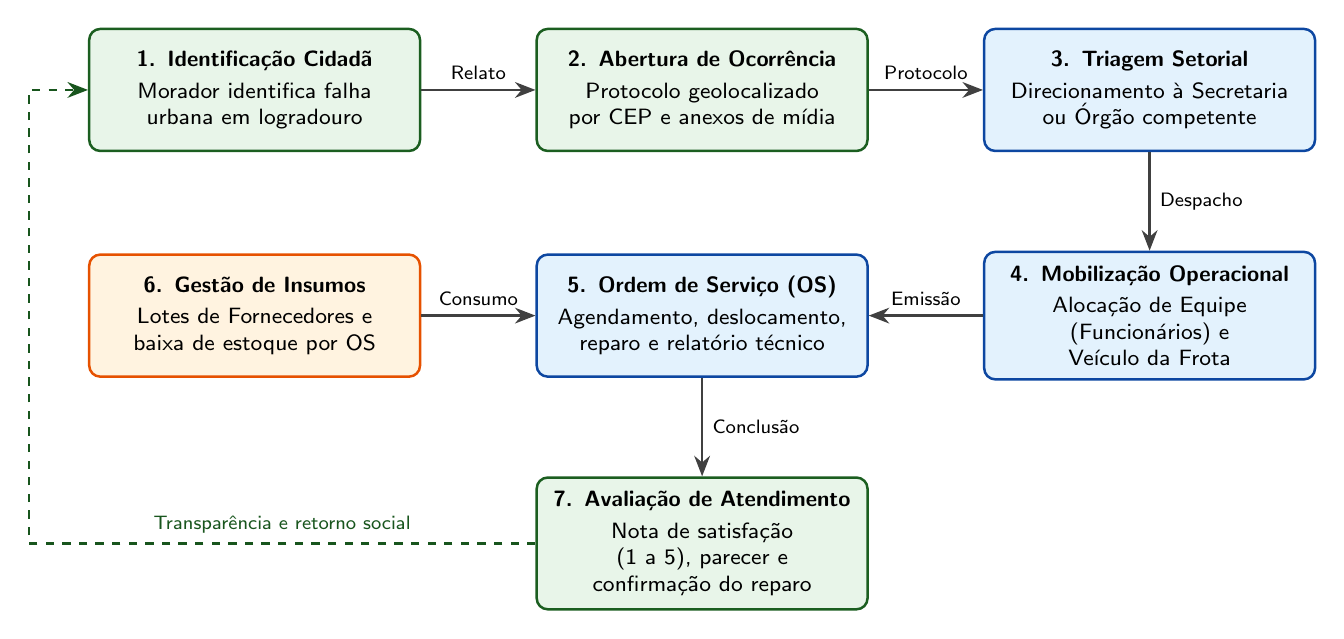
\begin{tikzpicture}[
    font=\sffamily\footnotesize,
    node distance=1.15cm and 1.45cm,
    blocoBase/.style={
        rectangle, rounded corners=4pt, line width=0.9pt,
        text width=3.85cm, minimum height=1.55cm,
        align=center, inner sep=5pt,
        execute at begin node={\hyphenpenalty=10000\exhyphenpenalty=10000}
    },
    blocoCid/.style={
        blocoBase, draw=corCidadao, fill=corFundoCid
    },
    blocoPref/.style={
        blocoBase, draw=corPrefeitura, fill=corFundoPref
    },
    blocoSup/.style={
        blocoBase, draw=corSuprimento, fill=corFundoSup
    },
    seta/.style={
        -{Stealth[length=2.6mm,width=2.0mm]}, line width=0.9pt, draw=black!75
    },
    setaRetorno/.style={
        -{Stealth[length=2.6mm,width=2.0mm]}, line width=0.9pt, dashed, draw=corCidadao!90!black
    }
]

% Linha 1: Demanda Cidadã e Triagem
\node[blocoCid] (n1) {\textbf{1. Identificação Cidadã}\\[2pt]Morador identifica falha urbana em logradouro};
\node[blocoCid, right=of n1] (n2) {\textbf{2. Abertura de Ocorrência}\\[2pt]Protocolo geolocalizado por CEP e anexos de mídia};
\node[blocoPref, right=of n2] (n3) {\textbf{3. Triagem Setorial}\\[2pt]Direcionamento à Secretaria ou Órgão competente};

% Linha 2: Mobilização, Execução e Suprimentos
\node[blocoPref, below=1.25cm of n3] (n4) {\textbf{4. Mobilização Operacional}\\[2pt]Alocação de Equipe (Funcionários) e Veículo da Frota};
\node[blocoPref, left=of n4] (n5) {\textbf{5. Ordem de Serviço (OS)}\\[2pt]Agendamento, deslocamento, reparo e relatório técnico};
\node[blocoSup, left=of n5] (n6) {\textbf{6. Gestão de Insumos}\\[2pt]Lotes de Fornecedores e baixa de estoque por OS};

% Linha 3: Conclusão e Auditoria Social
\node[blocoCid, below=1.25cm of n5] (n7) {\textbf{7. Avaliação de Atendimento}\\[2pt]Nota de satisfação (1 a 5), parecer e confirmação do reparo};

% Ligações principais
\draw[seta] (n1) -- node[above, font=\sffamily\scriptsize]{Relato} (n2);
\draw[seta] (n2) -- node[above, font=\sffamily\scriptsize]{Protocolo} (n3);
\draw[seta] (n3) -- node[right, font=\sffamily\scriptsize]{Despacho} (n4);
\draw[seta] (n4) -- node[above, font=\sffamily\scriptsize]{Emissão} (n5);
\draw[seta] (n6) -- node[above, font=\sffamily\scriptsize]{Consumo} (n5);
\draw[seta] (n5) -- node[right, font=\sffamily\scriptsize]{Conclusão} (n7);

% Linha de retorno social pela lateral esquerda sem colisão
\coordinate (cantoInfEsq) at ([xshift=-0.75cm]n6.west |- n7.west);
\coordinate (cantoSupEsq) at ([xshift=-0.75cm]n1.west);
\draw[setaRetorno] (n7.west) -- node[above, font=\sffamily\scriptsize, text=corCidadao!90!black]{Transparência e retorno social} (cantoInfEsq) -- (cantoSupEsq) -- (n1.west);

\end{tikzpicture}
\end{document}
